\section*{問題4}
\noindent
データが単位正方形の上で,一様分布に従うとすると,$R(C)$は図\ref{4-1}の着色部分の面積に等しい.
\begin{figure}[H]
    \begin{center}
        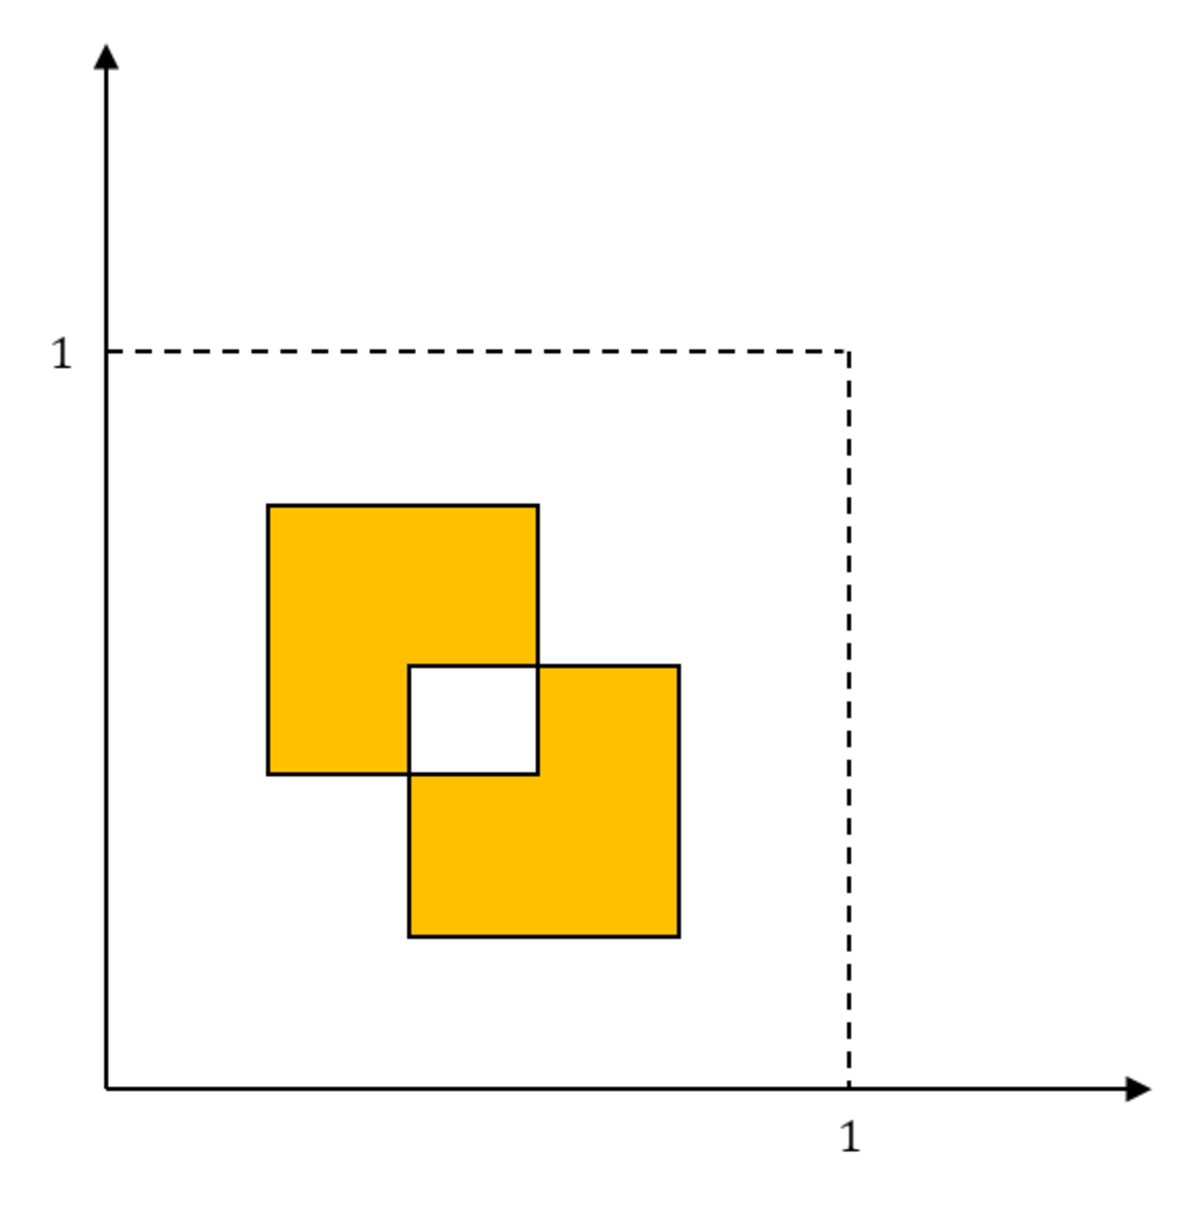
\includegraphics[width=100mm]{./figures/section_4/figure1.eps}
        \label{4-1}
    \end{center}
\end{figure}
次に,任意の長方形の上で一様に分布している場合の$R(C)$について考える.\\
図\ref{4-2}のように任意の長方形の横と縦の長さをそれぞれ$p$, $q$とおき,着色部分の面積を$S$とおくと
\begin{eqnarray*}
    R(C)=\frac{S}{pq}
\end{eqnarray*}
となる.
\begin{figure}[H]
    \begin{center}
        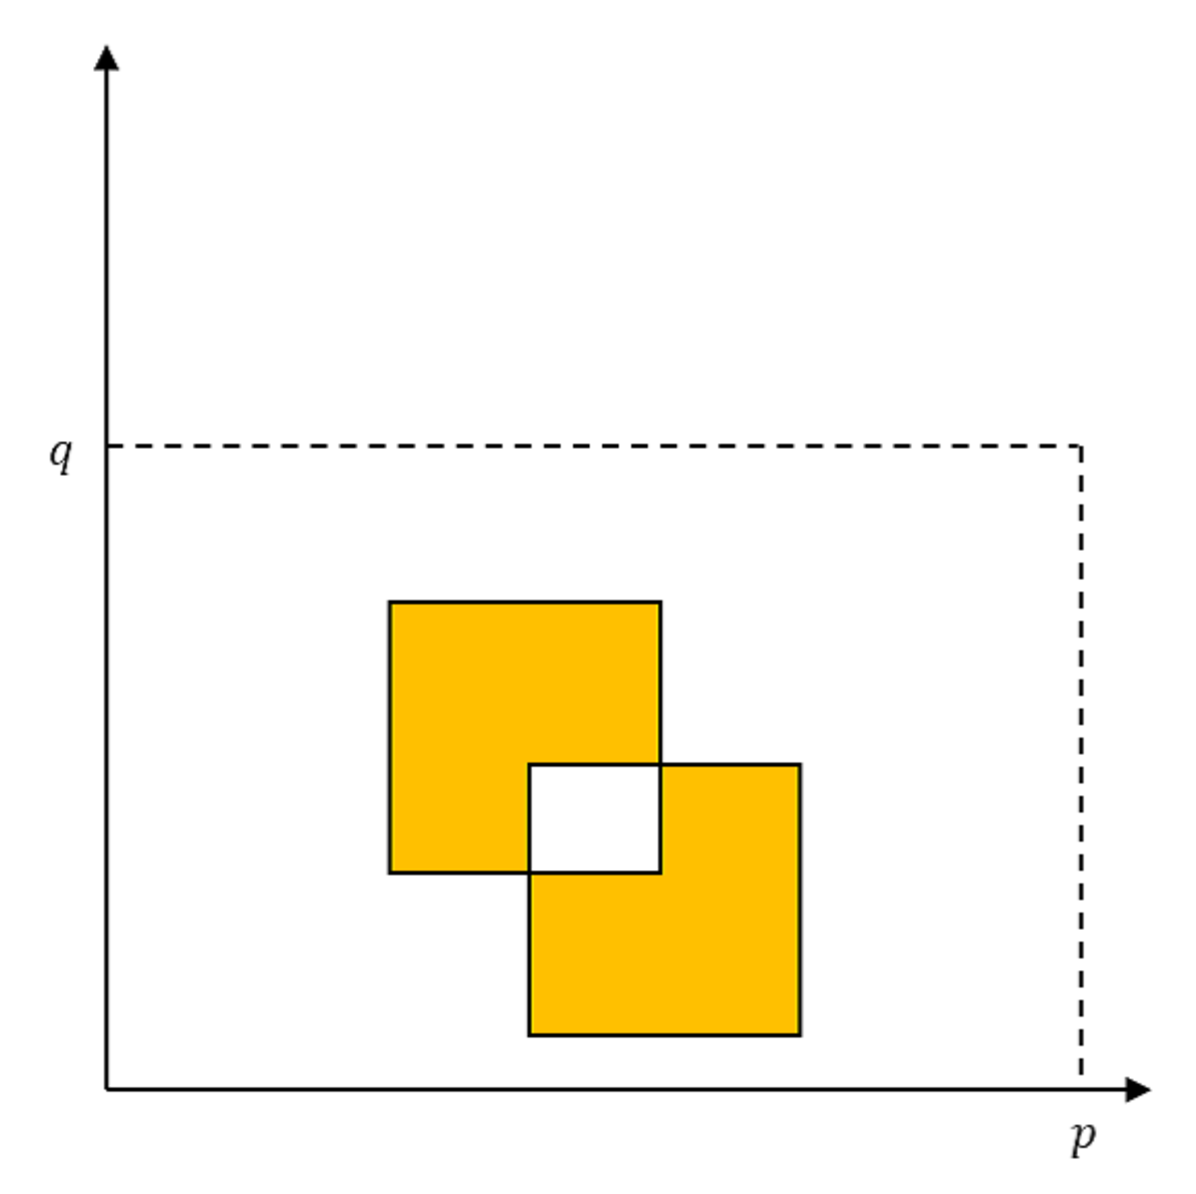
\includegraphics[width=100mm]{./figures/section_4/figure2.eps}
        \label{4-2}
    \end{center}
\end{figure}